\section{实验与结果}

实验针对于CNN与BiLSTM两种网络模型在同一数据集上,分别进行实验,验证模型效果。实验首先进行数据集预处理,随后分别进行CNN和BiLSTM中文情感分析模型的训练与评估。

这里我们使用NVIDIA Tesla V100 GPU训练基于CNN模型和BiLSTM的的中文情感预测模型。

\subsection{数据集预处理}

\begin{itemize}
    \item \textbf{step1:} 划分数据集\\
    本实验的数据集为4000条关于酒店的评论语料(来自谭松波老师的评论语料)。将原始数据集按照4:1的比例划分为训练集和测试集。共3200个样本的测试集与800个样本的验证集。数据集种已经标注好了标记(积极-POS,消极-NEG)。
    \item \textbf{step2:} 分词\\
    使用JieBa分词\cite{Jieba},对训练集与测试集分别进行分词,词与词之间空格分隔开。对分此后的语料,利用原始数据集标注好的标记为每一行都打上标记。
    \item \textbf{step3:} 提取词向量\\
    由于预训练的词向量非常庞大,我们需要预先提取训练语料中出现的字符对应的向量。
\end{itemize}

\subsection{基于CNN模型的中文情感预测}

首先使用提取后的词向量对语料库Embedding,形成单通道,传给CNN中文情感预测模型,进行模型训练。使用训练集训练模型,并使用测试集测试模型推理性能。训练的关键参数如表\ref{tab:cnn_training_parameters}。

\begin{table}[H]
    \centering
    \begin{tabular}{c@{\hspace{40pt}}c}
        \toprule
        \textbf{Parameter} & \textbf{Value} \\
        \midrule
        dim& 300\\
        nwords& 300 \\
        filter\_sizes& [2, 3, 4]\\
        num\_filters& 64\\
        dropout & 0.6\\
        num\_oov\_buckets & 1\\
        epochs & 50\\
        batch\_size & 20\\
        buffer & 3500\\
        \bottomrule
    \end{tabular}
    \caption{CNN中文情感预测模型训练参数}
    \label{tab:cnn_training_parameters}
\end{table}


训练完成后,我们得到了训练好的基于CNN的中文情感分析模型。

接下来,进行模型评估。我们从准确率、召回率与F1-score三个指标分析模型性能。模型性能评估结果如图\ref{fig:cnnres}所示。

\begin{figure}[H]
    \centering
    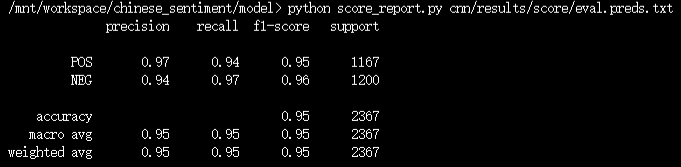
\includegraphics[width=0.9\linewidth]{sections//fig/cnn_res.png}
    \caption{CNN模型的训练结果}
    \label{fig:cnnres}
\end{figure}

最后,导出我们训练好的模型,进行自主输入测试。基于CNN的中文情感分析模型测试结果如图\ref{fig:cnn_test}。

\begin{figure}[H]
    \centering
    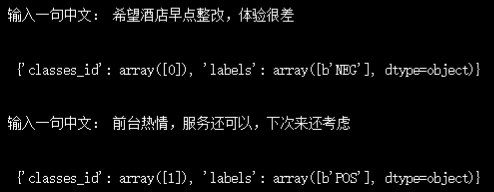
\includegraphics[width=0.9\linewidth]{sections//fig/cnn_test.png}
    \caption{CNN模型的测试结果}
    \label{fig:cnn_test}
\end{figure}

\subsection{基于BI-LSTM模型的中文情感预测}

首先,对分词后的语料样本进行Embedding,传入我们搭建好的BiLSTM模型中,进行模型训练。根据最后对模型输出的Logits进行Softmax操作,得到情感分析的结果的概率,与原标记比较。模型训练参数如表\ref{tab:bilstm_training_parameters}。

\begin{table}[H]
    \centering
    \begin{tabular}{c@{\hspace{40pt}}c}
        \toprule
        \textbf{Parameter} & \textbf{Value} \\
        \midrule
        dim & 300\\
        channel & 32\\
        dropout & 0.5\\
        num\_oov\_buckets & 1\\
        epochs & 25\\
        batch\_size & 20\\
        buffer & 3500\\
        \bottomrule
    \end{tabular}
    \caption{BiLSTM中文情感预测模型训练参数}
    \label{tab:bilstm_training_parameters}
\end{table}

进行多轮训练后,对训练好的模型进行评估。评价指标同基于CNN的中文情感分析模型(准确率、召回率与F1-score)。模型性能评估结果如图\ref{fig:bires}所示。

\begin{figure}[H]
    \centering
    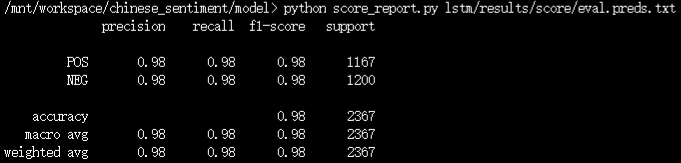
\includegraphics[width=0.9\linewidth]{sections//fig/bi_res.png}
    \caption{BI-LSTM模型的训练结果}
    \label{fig:bires}
\end{figure}

最后,导出我们训练好的模型,进行自主输入测试。基于BiLSTM的中文情感分析模型测试结果如图\ref{fig:bilstm_test}。

\begin{figure}[H]
    \centering
    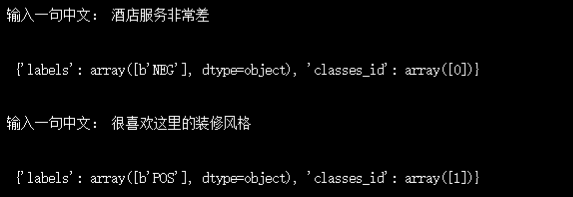
\includegraphics[width=0.9\linewidth]{sections//fig/bilstm_test.png}
    \caption{BiLSTM模型的测试结果}
    \label{fig:bilstm_test}
\end{figure}

\vspace{2em}

综上所述,我们分别采用CNN和BI-LSTM两种模型解决文本分类任务,并用于情感分析,达到不错的效果。 CNN模型在小数据集上训练,在验证集的准确率、号回率及F1因子均接近95\%。BI-LSTM模型,在验证集的准确率、号回率及F1因子均接近98\%。